\documentclass[aspectratio=169,xcolor=table]{beamer}
\usepackage{algorithm}
\usepackage{algpseudocode}
\usepackage[utf8]{inputenc}
\usepackage[T1]{fontenc}
\usepackage{lipsum, lmodern}
\usepackage{csquotes}
\usepackage{xcolor}
\usepackage[portuguese]{babel}
\usepackage{amsmath}
\usepackage{physics}

% ------------------------------------------------
% Tema do Beamer (exemplo de um tema customizado)
% ------------------------------------------------
\usetheme{DCC} % <-- Ajuste conforme seu tema ou estilo

\graphicspath{{imgs/}{./imgs/}}

\author[Magalhães, Felipe]{%
  \textbf{Antoniel Magalhães} \\
  \textbf{Luis Felipe}
}
\title{Simulação de ondas e oceano}
\institute{Universidade Federal da Bahia \\ Instituto de Computação}
\date{\today}

\begin{document}

%-------------------------------------------------
%  SLIDE DE TÍTULO
%-------------------------------------------------
\begin{frame}[plain,noframenumbering]
    \titlepage
\end{frame}

%-------------------------------------------------
%  SLIDE DE AGENDA
%-------------------------------------------------
\begin{frame}{Agenda}
    \tableofcontents
\end{frame}

\setlength{\parskip}{1em} % Adjust the space between paragraphs

%=================================================
\section{Introdução}
%=================================================
\begin{frame}{Introdução}
    \begin{itemize}
        \item A simulação de ondas e oceano é uma área de estudo que combina física, matemática e computação para modelar o comportamento das ondas no mar.
        \item Este campo é crucial para:
        \begin{itemize}
            \item Jogos e aplicações interativas
            \item Efeitos visuais em filmes e animações
            \item Visualização científica
            \item Simuladores de treinamento marítimo
        \end{itemize}
    \end{itemize}
\end{frame}

%=================================================
\section{Fundamentos Físicos}
%=================================================
\begin{frame}{Fundamentos da Teoria Linear}
    \begin{itemize}
        \item Baseada na Teoria Linear de Ondas (Airy, 1845)
        \item Simplificações importantes para computação gráfica:
        \begin{itemize}
            \item Fluido homogêneo e incompressível
            \item Tensão superficial desprezada
            \item Fundo plano e horizontal
        \end{itemize}
        \item Estas simplificações permitem implementações eficientes mantendo realismo visual \cite{meirelles2007modelagem}
    \end{itemize}
\end{frame}

\begin{frame}{Pressupostos da Teoria Linear}
    \begin{itemize}
        \item A teoria linear assume que: o fluido é homogêneo, incompressível (densidade constante) e irrotacional.
        \item A tensão superficial é desprezada.
        \item A pressão na superfície livre é uniforme e constante.
        \item O fluido é invíscido.
        \item O fundo é um limite plano, horizontal, fixo e impermeável.
    \end{itemize}
\end{frame}

\begin{frame}{Aspectos Computacionais}
    \begin{itemize}
        \item Na computação gráfica, a superfície da água é frequentemente representada como uma malha de vértices
        \item A elevação da superfície $\eta(x,t)$ é dada por:
        \[\eta(x,t) = \frac{H}{2}\cos(kx-\omega t)\]
        \item A relação de dispersão conecta frequência e número de onda:
        \[\omega^2 = gk\tanh(kh)\]
    \end{itemize}
\end{frame}

\begin{frame}{Técnicas de Renderização}
    \begin{itemize}
        \item Métodos de renderização em tempo real:
        \begin{itemize}
            \item Normal mapping para detalhes da superfície
            \item Fresnel effect para reflexão/refração
            \item Caustics para efeitos de luz subaquática
        \end{itemize}
        \item A velocidade das partículas é dada por:
        \[\vec{v} = \nabla\phi = \begin{pmatrix}
            \frac{\partial \phi}{\partial x} \\
            \frac{\partial \phi}{\partial z}
        \end{pmatrix}\]
    \end{itemize}
\end{frame}

\begin{frame}{Técnicas de Otimização}
    \begin{itemize}
        \item Level of Detail (LOD):
        \begin{itemize}
            \item Malha adaptativa baseada na distância
            \item Redução de vértices em áreas distantes
        \end{itemize}
        \item Otimizações de renderização:
        \begin{itemize}
            \item Frustum culling
            \item Vertex buffer optimization
            \item Shader optimizations
        \end{itemize}
        \item Performance em tempo real \cite{wavesimulator2024}
    \end{itemize}
\end{frame}

%=================================================
\section{Simulação do Empinamento}
%=================================================
\begin{frame}{Simulação do Empinamento}
    \begin{itemize}
        \item O empinamento das ondas é um fenômeno importante na dinâmica oceânica.
        \item A simulação deste processo ajuda a entender como as ondas interagem com estruturas costeiras e como a energia das ondas é dissipada.
    \end{itemize}
\end{frame}

%=================================================
\section{Computação Gráfica na Simulação de Ondas}
%=================================================
\begin{frame}{Computação Gráfica na Simulação de Ondas}
    \begin{itemize}
        \item A computação gráfica desempenha um papel vital na visualização das simulações de ondas.
        \item Técnicas avançadas permitem a criação de modelos visuais realistas que ajudam na análise e interpretação dos dados simulados.
    \end{itemize}
\end{frame}

%=================================================
\section{Implementação em Three.js}
%=================================================
\begin{frame}{Simulação em Three.js}
    \begin{itemize}
        \item Three.js: biblioteca JavaScript para computação gráfica 3D \cite{threejs2024}
        \item Componentes principais:
        \begin{itemize}
            \item Geometria: PlaneGeometry para superfície da água
            \item Material: MeshPhongMaterial para reflexões realistas
            \item Iluminação: Combinação de luzes direcionais e ambiente
        \end{itemize}
    \end{itemize}
\end{frame}

\begin{frame}{Demonstração da Simulação}
    \begin{center}
        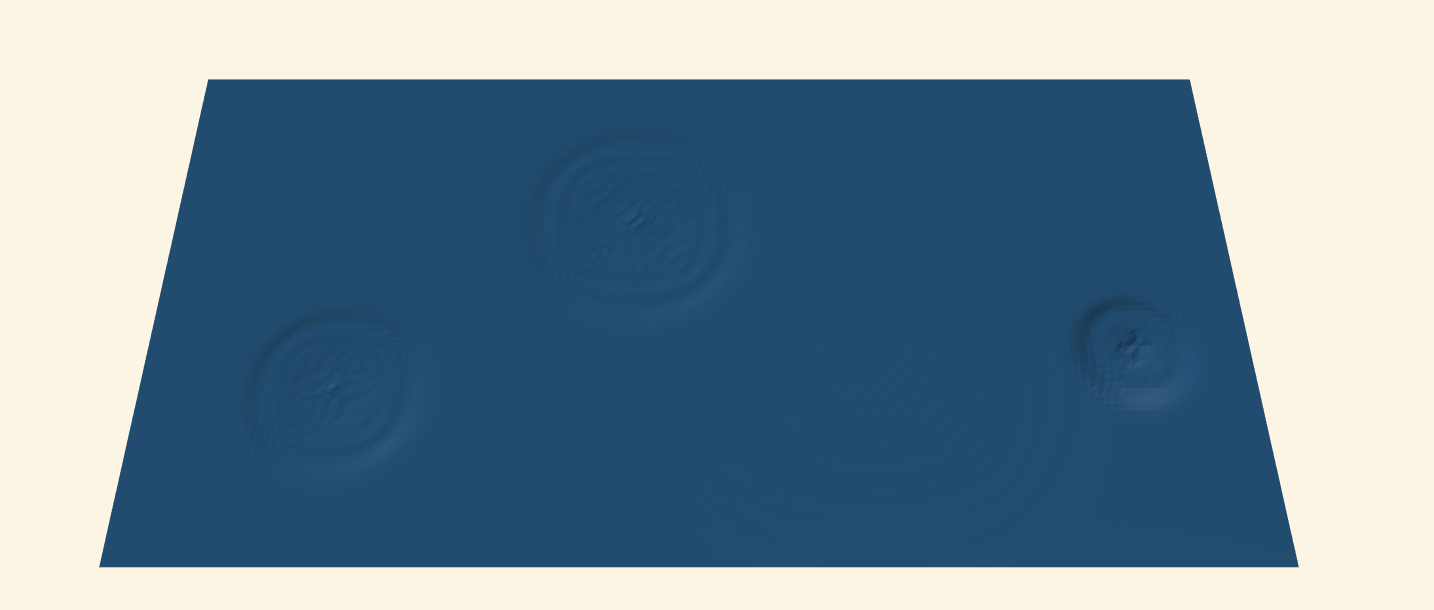
\includegraphics[height=0.35\textheight]{imgs/wave.png}
    \end{center}
    
    \begin{itemize}
        \item Simulação de ondas em tempo real usando Three.js
        \item Demonstração completa: \href{https://github.com/alephoverflow/WaveSimulator}{GitHub}
    \end{itemize}
\end{frame}

\begin{frame}[fragile]{Modelo de Propagação de Ondas}
    \begin{itemize}
        \item Modelo baseado em sistema de molas para simulação de ondas:
    \end{itemize}
    \begin{verbatim}
class PropagationSpringModel {
    constructor(rows, columns) {
        this.heightField = new Float32Array(rows * columns);
        this.velocityField = new Float32Array(rows * columns);
        
        // Constantes físicas da simulação
        this.springConstant = 0.008;  // Elasticidade
        this.damping = 0.025;         // Amortecimento
        this.propagationSpeed = 5.0;   // Velocidade
    }
}
    \end{verbatim}
\end{frame}

\begin{frame}[fragile]{Renderização com Three.js}
    \begin{itemize}
        \item Configuração básica da cena 3D:
    \end{itemize}
    \begin{verbatim}
class OceanSimulation {
    constructor() {
        this.scene = new THREE.Scene();
        this.camera = new THREE.PerspectiveCamera(45);
        
        // Material realista para água
        this.waterMaterial = new THREE.MeshPhongMaterial({
            color: 0x006994,
            specular: 0x111111,
            shininess: 40
        });
    }
}
    \end{verbatim}
\end{frame}

%=================================================
\section{Técnicas Avançadas de Simulação}
%=================================================
\begin{frame}{Survey: Estado da Arte em Simulação de Oceanos}
    \begin{itemize}
        \item Survey de técnicas de simulação \cite{darles2011survey}:
        \begin{itemize}
            \item Métodos baseados em física
            \item Métodos de domínio espacial
            \item Técnicas híbridas para melhor performance
        \end{itemize}
        \item Desafios identificados no survey:
        \begin{itemize}
            \item Equilíbrio entre realismo e performance
            \item Simulação de fenômenos complexos
            \item Integração com sistemas em tempo real
        \end{itemize}
    \end{itemize}
\end{frame}

\begin{frame}{Survey: Técnicas Avançadas}
    \begin{itemize}
        \item Método Euleriano baseado em física \cite{thurey2007realtime}:
        \begin{itemize}
            \item Simulação em tempo real de águas rasas
            \item Modelagem realista de ondas quebrando
            \item Otimizado para GPU
        \end{itemize}
        \item Técnicas modernas de GPU \cite{bonaventura2018terrain}:
        \begin{itemize}
            \item Tesselação dinâmica da superfície
            \item Nível de detalhe adaptativo
            \item Otimização de geometria em tempo real
        \end{itemize}
    \end{itemize}
\end{frame}

%=================================================
\section{Referências}
%=================================================
\begin{frame}[allowframebreaks]{Referências}
    \bibliographystyle{plain}
    \bibliography{Bibliografia}
\end{frame}

\end{document}
